\documentclass[10pt,letterpaper]{article}
\usepackage[utf8]{inputenc}
\usepackage{amsmath}
\usepackage{amsfonts}
\usepackage{amssymb}

\usepackage[margin=0.5in]{geometry}		%used for margins
\usepackage{graphicx}					%used for images
\usepackage{booktabs}					%used for nicer tables
\pagenumbering{gobble}					%suppress page numbers

\title{Functional Testing - Decision Tables}
\author{
	Cai, Zelin\\
	\and
	Silvestre, Patrick\\
}
\date{}

\begin{document}
\maketitle
\newpage
\section{Workflow Diagram}
\begin{figure}[h]
	\centerline{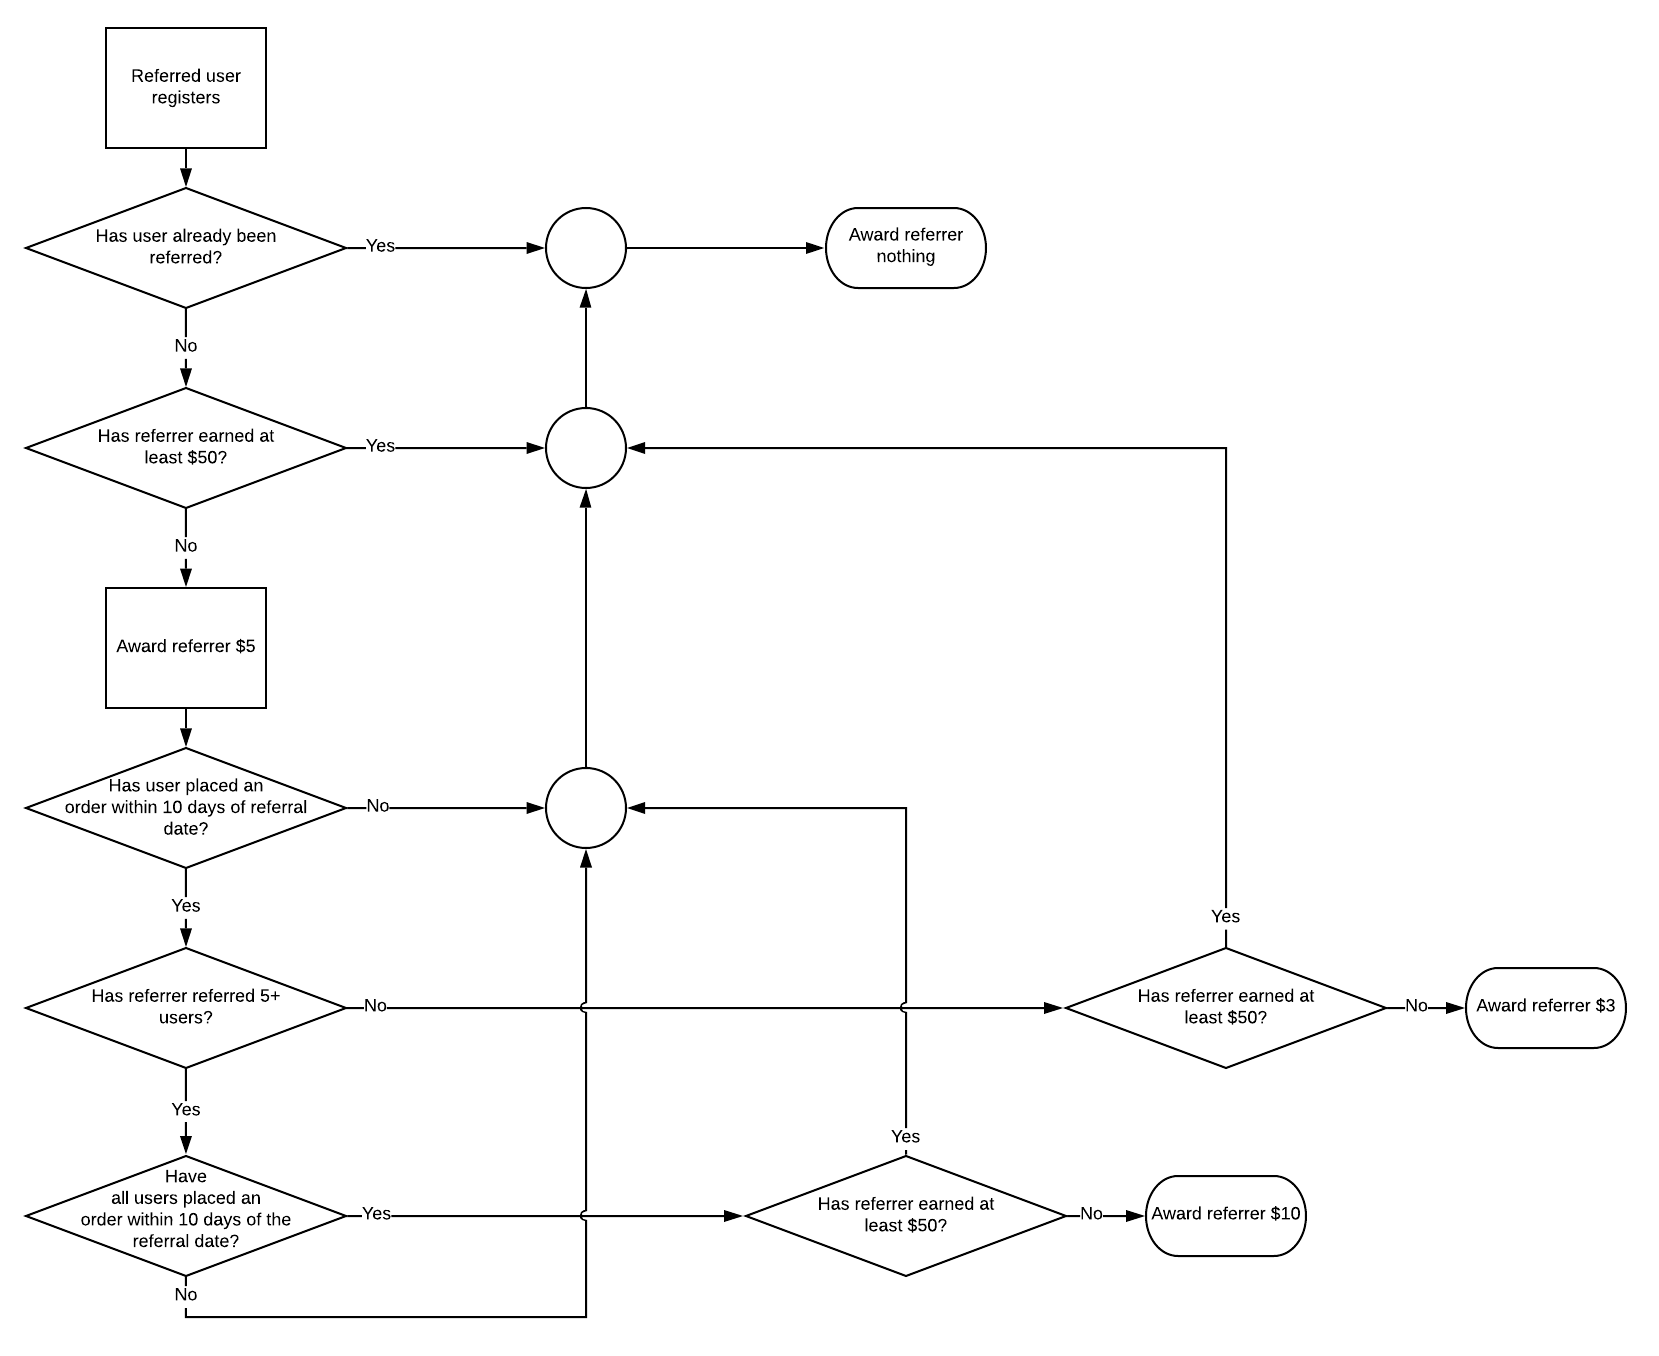
\includegraphics[width=9.5cm]{workflow.png}}
\end{figure}

\newpage
\section{Decision Table (After Column Reduction)}
\begin{table}[h]
\centerline{
\begin{tabular}{@{}lllllll@{}}
\toprule
                                                                     &                 & \multicolumn{5}{c}{\textbf{Rules or Combinations}}             \\ \cmidrule(l){3-7} 
\textbf{Conditions}                                                  & \textbf{Values} & \textbf{1} & \textbf{2} & \textbf{3} & \textbf{4} & \textbf{5} \\ \midrule
$C_1$: User is already referred                                             & Y, N            & Y          & N          & N          & N          & N          \\
$C_2$: Referrer has earned at least \$50                                    & Y, N            & —          & Y          & N          & N          & N          \\
$C_3$: Referred user places an order within 10 days                         & Y, N            & —          & —          & N          & Y          & Y          \\
$C_4$: Referrer has referred 4+ additional users and all place an order within 10 days & Y, N            & —          & —          & —          & N          & Y          \\
\textbf{Effects}                                                     &                 &            &            &            &            &            \\
$E_1$: Award referrer nothing                                               &                 & 1          & 1          &            &            &            \\
$E_2$: Award referrer \$5                                                   &                 &            &            & 1          & 1          & 1          \\
$E_3$: Award referrer \$3                                                   &                 &            &            &            & 2          & 2          \\
$E_4$: Award referrer \$10                                                  &                 &            &            &            &            & 3          \\ \bottomrule
\end{tabular}
}
\end{table}

\section{Scenarios}
\subsection{Scenario 1}
Suppose:
\begin{itemize}
	\item{User is already referred}
	\item{Referrer has not earned at least \$50}
	\item{Referred user places an order within 10 days}
	\item{Referrer has not referred 4+ additional users}
\end{itemize}
Using the decision table, this scenario falls under rule 1. $C_1$ is true, and the remaining conditions do not have an impact on the final effect: $E_1$.

\subsection{Scenario 2}
Suppose:
\begin{itemize}
	\item{User is not already referred}
	\item{Referrer has earned at least \$50}
	\item{Referred user places an order within 10 days}
	\item{Referrer has not referred 4+ additional users}
\end{itemize}
Using the decision table, this scenario falls under rule 2. $C_1$ is false, $C_2$ is true, and the remaining conditions do not have an impact on the final effect: $E_1$.

\subsection{Scenario 3}
Suppose:
\begin{itemize}
	\item{User is not already referred}
	\item{Referrer has not earned at least \$50}
	\item{Referred user does not place an order within 10 days}
	\item{Referrer has not referred 4+ additional users}
\end{itemize}
Using the decision table, this scenario falls under rule 3. $C_1$, $C_2$, and $C_3$ are false, and the remaining condition does not have an impact on the final effect: $E_2$.

\end{document}